\documentclass[a4paper,11pt]{article}

\usepackage{Style/thesis}



\begin{document}

\title{\Huge{Animal Shelter Outcomes\footnote{Kaggle competition available at \url{https://www.kaggle.com/c/shelter-animal-outcomes}}}\\
	\LARGE{Data Mining Project}}
\author{\Large{PoliKagglers}\\ \\
	Alberto Donizetti\footnote{\href{mailto:alberto.donizetti@mail.polimi.it}{alberto.donizetti@mail.polimi.it}}, Alessandro Negrini, Enrico Bertino,\\ Marta Toschi, Pierpaolo Necchi}
\maketitle

\section{Introduction}
Every year, approximately 7.6 million companion animals end up in US shelters. Many of these animals find forever families to take them home, but just as many are not so lucky: 2.7 million dogs and cats are euthanized in the US every year. The ``Animal Shelter Outcomes'' Kaggle competition goal is to predict the outcome for each animal given a dataset of intake information. Understanding trends in outcomes could help shelters focusing on specific animals who need a little extra help finding a new home.  

\section{Data Exploration}
The initial phase of our work consisted in a qualitative analysis of the dataset: we tried to discover meaningful patterns and correlations among variables in order to distinguish between relevant and irrelevant features. For instance, Figure \ref{fig:sex_patterns} shows the dependence between the animal gender and the outcome. We notice that the majority of the animals being adopted or returned to the owner are neutered: this pattern may be due to a shelter policy or to the US law but provides a strong predictor of adoptions or returns. Figure \ref{fig:hourly_patterns} shows the hourly distribution of outcomes and we clearly spot some interesting patterns that can be successfully exploited during classification. For example, transfers are particularly frequent around 0:00 and 9:00, which again may be due to the shelter policy. Similarly, adoptions frequently occur between 17:00 and 18:00.

\begin{figure}[t]
\centering
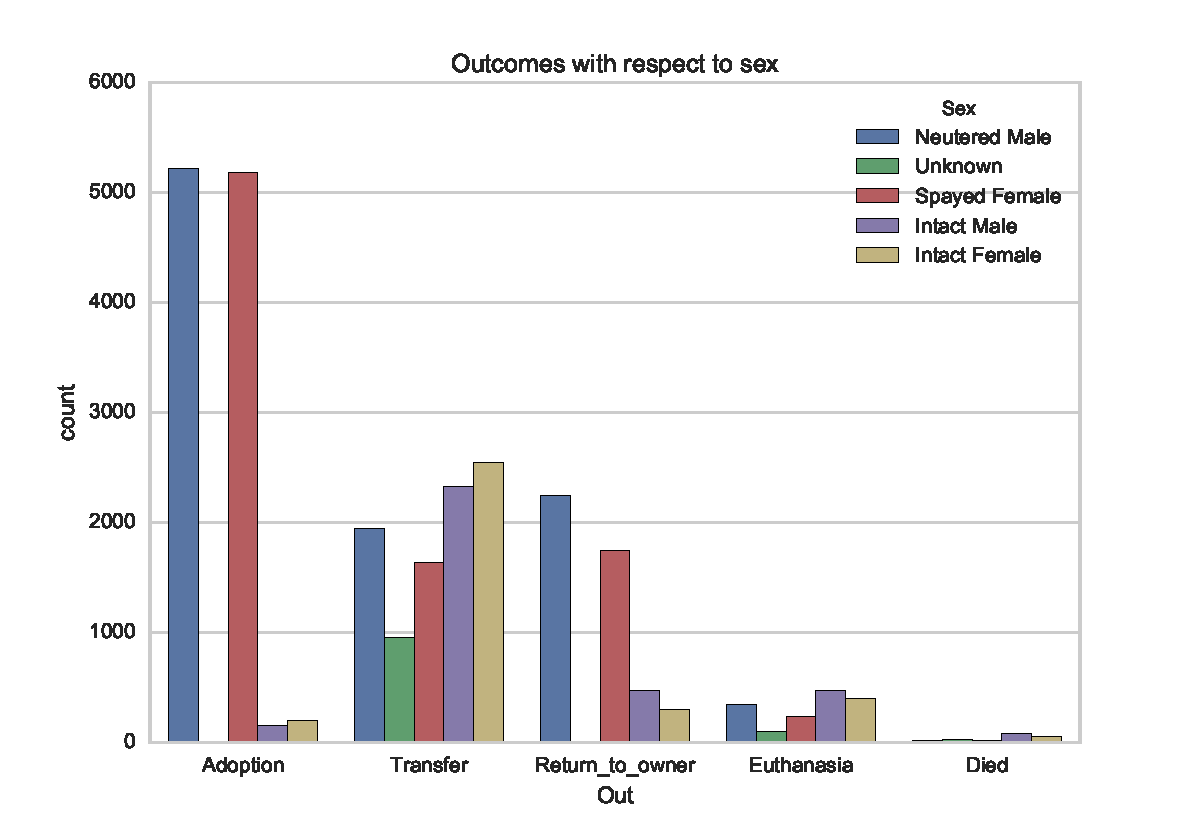
\includegraphics[width=.9\linewidth]{./figure_2}
\caption{Dependence between the animal status and the outcome.}
\label{fig:sex_patterns}
\end{figure}

\begin{figure}[h!]
\centering
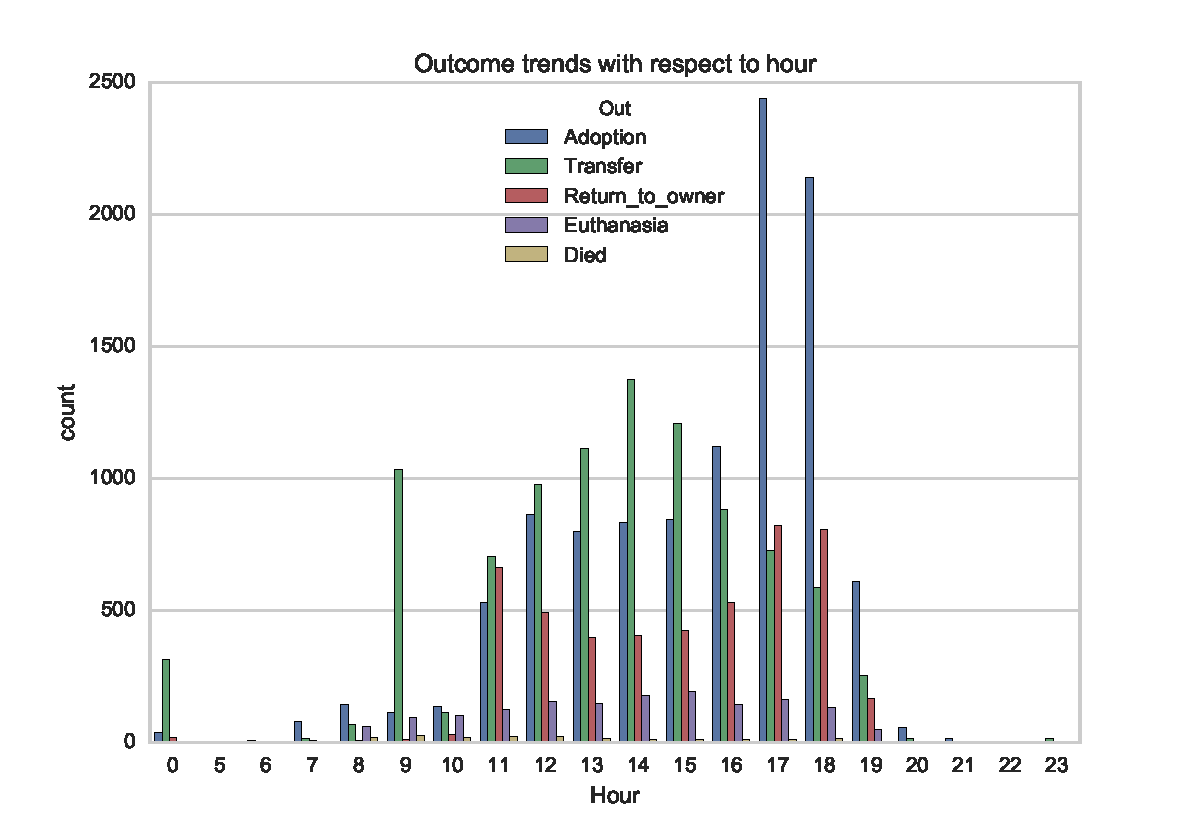
\includegraphics[width=.9\linewidth]{./figure_4}
\caption{Hourly patterns in outcome types.}
\label{fig:hourly_patterns}
\end{figure}

\section{Dealing with leaks}
Thanks to this exploratory analysis, we spotted two criticalities in the dataset that greatly affected the project. The first one is that the data provided depicts the state of the animals at the outcome time and not at the intake time. Hence, some variables present a larger than expected correlation with the outcome type. For instance, since animals are often sterilized before being adopted or transfered, the status of the animal is of great importance in predicting these outcomes. The second criticality is that the training set and the test set cover the exact same period and, subsequently, times greatly improve prediction accuracy since they can be used to predict blocks of outcomes of the same type. This overlapping in time seems to contradict one of the competition rules, which states that a ``model should only use information which was available prior to the time for which it is forecasting''. This rule would make sense if the test set covered times following those of the training set but, because of this overlapping, it would become computationally difficult to abide by it. Like most of the participants, we thus decided to neglect this rule and use the whole training set to build our model. This assumption and the criticalities discussed above forced us to consider two different approaches: a first one taking advantage of the leak between training and test set and a second one which does not exploit it. 


\section{Preprocessing and Feature Engineering}
During the preprocessing step, most of the variables provided in the original dataset had to be transformed to a format compatible with the classification libraries used to predict the outcomes. Moreover, the aggregate attributes such as DateTime were split in more granular features, such as year, month, day, hour. In doing so, it was necessary to identify which variables exploited the leak between training and test set discussed in the previous section. The original features and the attributes obtained during the preprocessing are summarized in Table \ref{tab:features}.\\
In addition to trivial transformations, we introduced a set of features which measures if a certain outcome belongs to a cluster of outcomes of a certain type. These variables try to directly exploit the fact that many outcomes of the same type happen in blocks highly concentrated in time and, because of the overlapping between training and test set, they appear to be very powerful predictors. 

\begin{table}[t]
\centering
\begin{tabular}{@{}lllll@{}}
\toprule
Original Variable & Type        & Variables obtained & Type        & Leak \\ \midrule
Name             & String      & Length of name     & Numerical   & No   \\
Date and time    & Datetime    & Year               & Numerical   & Yes  \\
                 &             & Season             & Numerical   & No   \\
                 &			   & Holidays			& Categorical & No \\
                 &             & Month              & Numerical   & No   \\
                 &             & Day of week        & Numerical   & No   \\
                 &             & Day                & Numerical   & Yes  \\
                 &             & Day of year        & Numerical   & Yes  \\
                 &             & Hour               & Numerical   & Yes  \\
                 &             & Minute             & Numerical   & Yes  \\
                 &             & Minute of day      & Numerical   & Yes  \\
                 &             & Outcomes clusters  & Numerical   & Yes  \\
Animal type      & Categorical & Animal Type        & Categorical & No   \\
Sex upon outcome & Categorical & Gender             & Categorical & No   \\
                 &             & Status             & Categorical & Yes  \\
Age upon outcome & Ordinal     & Age in days        & Numerical   & No   \\
		&	   & GroupAges		& Categorical & No\\
Breed            & Categorical & Breed Groups       & Categorical & No   \\
                 &             & Mix and multibreed & Categorical & No   \\
                 &             & Dangerous          & Categorical & No   \\
Color            & Categorical & Number of colors   & Numerical   & No   \\
                 &             & Color groups       & Categorical & No   \\
                 &             & Pattern            & Categorical & No   \\ \bottomrule
\end{tabular}
\caption{Original features and features built for the classification process in the leak and no-leak cases.}
\label{tab:features}
\end{table}

\section{Classification}
The goal of this competition is to predict, for each animal, the probabilities of belonging to each of the five classes Adoption, Died, Euthanasia, Return to owner and Transfer. The problem so defined puts us in a multi-class classification framework in which the accuracy of a classifier is evaluated using the multi-class logarithmic loss metric. The literature offers several algorithms able to deal with multi-class classification and some considerations have to be made in order to choose a well-suited method. In particular, the presence of both categorical and numerical attributes drove us to only consider two classification methods that usually perform well out-of-the-box: \emph{random forests} and \emph{gradient boosting trees} classifiers. Conversely, algorithms such as logistic regression, support vector machines, neural networks and k-nearest neighbors have been discarded due to their low capability of handling data of ``mixed'' type and of identifying irrelevant inputs \cite{friedman2009elements}. 

\subsection{Software and Tools}
The entire classification pipeline for this competition has been implemented in Python, exploiting some powerful external libraries such as 
\begin{enumerate}
	\item \textit{Pandas} which provides high-performance and easy-to-use data structures and data analysis tools.
	\item \textit{Scikit-learn}\cite{scikit-learn} which provides an efficient implementation of the random forest classifier and some useful tools for model validation.
	\item \textit{Xgboost}\cite{chen2015xgboost} which provides a state-of-the-art implementation of a gradient boosting tree classifier, which is very popular and successful in Kaggle competitions.  
\end{enumerate}

\subsection{Model Validation}
Random forests and the xgboost classifiers typically work well out-of-the-box, but a careful tuning of their parameters can yield large improvements in classification accuracy. In order to evaluate the performances of our classifiers and select the best combination of parameters, we used a fairly standard model validation procedure. First, using an 80/20 split of the training set, we extracted a validation set on which we computed several accuracy metrics, such as the precision, recall, F1-score and logloss. To avoid overfitting the training set with the xgboost classifier, we used the early stopping regularization technique, which consists in training the classifier as long as the logloss score on the validation set hasn't decreased for a certain number of learning steps and then use the classifier which corresponds to the minimum validation error. Finally, we used a grid search approach exploiting cross-validation to select the best set of parameters for the booster.\\
Table \ref{tab:xgboost_performance_leak} reports some performance scores for the xgboost classifier with and without the leak exploitation. We don't report the results of the random forest since they were generally worse than those obtained with xgboost. We clearly see that exploiting the leak has a large positive impact on the classification of all the five classes. In particular, the leak yields a large improvement on the Died and Euthanasia classes, that were poorly or never predicted without exploiting it because of their small support and the poor predictive power of no-leak features.\\
Xgboost and random forests allow to compute some scores of feature importance, which has been extremely useful during the feature selection phase. These scores highlight the importance of the leak variables, which all rank in the first positions. We don't report these scores for brevity. Finally, in order to reduce the variance of the xgboost classifier induced by the random holdout split, initialization and learning procedure, we used bagging to average the predictions of 10 different xgboost classifiers.

\begin{table}[t]
\centering
\begin{tabular}{@{}lrrrr@{}}
\toprule
                & Precision   & Recall      & F1-score    & Support \\ \midrule
Adoption        & 0.61 / 0.74 & 0.74 / 0.87 & 0.67 / 0.80 & 2154    \\
Died            & 0.00 / 0.69 & 0.00 / 0.28 & 0.00 / 0.40 & 39      \\
Euthanasia      & 0.60 / 0.71 & 0.16 / 0.46 & 0.25 / 0.56 & 311     \\
Return to owner & 0.43 / 0.54 & 0.47 / 0.49 & 0.45 / 0.52 & 957     \\
Transfer        & 0.69 / 0.88 & 0.59 / 0.80 & 0.63 / 0.84 & 1881    \\ \midrule
Average / Total & 0.60 / 0.75 & 0.60 / 0.75 & 0.59 / 0.74 & 5342    \\ \bottomrule
\end{tabular}
\caption{Performance metrics on the validation set for the xgboost classifier without and with the leak exploitation.}
\label{tab:xgboost_performance_leak}
\end{table}

\subsection{Results Analysis}
Table \ref{tab:milestones} reports the score progression and the corresponding ranking in the public leaderboard obtained by adding new variables and increasing the level of exploitation of the leak. It is easy to see the benefit in classification accuracy due to the animal status and time information, which are the most critical attributes. Moreover, it is clear that it would have been impossible to rank high in this competition without exploiting the leak, as most of the participants in the top positions was using it. 


\begin{table}[t]
\centering
\begin{tabular}{@{}lll@{}}
\toprule
Description                                      & Score   & Leaderboard \\ \midrule
Bagged xgboost classifier with no leak           & 0.91586 & 667         \\
Added animal status                              & 0.81768 & 454         \\
Added day, hour and minute information           & 0.69699 & 21          \\
Added outcome clusters                           & 0.64574 & 3           \\
Tuned xgboost parameters by grid search          & 0.62799 & 3           \\
Hierarchical xgboost \& random forest classifier & 0.62713 & 3           \\ \bottomrule
\end{tabular}
\caption{Project milestones.}
\label{tab:milestones}
\end{table}

\section{Conclusions and Further Developments}
In this Kaggle competition, we addressed a multi-class classification problem in which we had to predict the outcome for several shelter animals. Thanks to a thorough feature engineering and to a careful tuning of an \emph{xgboost} classifier, a state-of-the-art implementation of a gradient boosting trees classifier, we were able to reach the third position world-wide. We think there is still some room for improvement and we identified some possible research directions, which unfortunately we were not able to investigate further due to a lack of time.\\
First, we observed that the outcome ``return to owner'' is not easily distinguished from ``adoption'', so we think we could improve the performance of our classifier by learning how to better separate these two classes. \\
Secondly, we thought of combining different kinds of classifiers able to learn different aspects of the dataset. For instance, we tried using a random forest classifier to predict the instances on which the xgboost classifier was uncertain among two or more classes. Our first tests produces small gains in score but we think there is some improvement potential in this direction.\\
Finally, we tried to exploit the information related to the outcome subtype that we had previously excluded for the sake of simplicity. We thought we could use them to refine a subset of our predictions with a \emph{2-steps} classifier, but, mostly due to a lack of time, we could not obtain any significant improvement.\\

\nocite{*}
\bibliographystyle{acm}
\bibliography{Bibliography/bibliography}


	


\end{document}
